
\chapter{Data Flow Diagram and Use Case Diagram}

\noindent 
\paragraph{\Large{Introduction}}

\noindent\\ \textbf{ Data Flow Diagram (DFD)} graphically representing the functions, or processes, which capture, manipulate, store, and distribute data between a system and its environment and between components of a system. The visual representation makes it a good communication tool between User and System designer. Structure of DFD allows starting from a broad overview and expand it to a hierarchy of detailed diagrams. DFD has often been used due to the following reasons:
\noindent 

\begin{enumerate}
\item  Logical information flow of the system.

\item  Determination of physical system construction requirements.

\item  Simplicity of notation.

\item  Establishment of manual and automated systems requirements.
\end{enumerate}

\noindent 
\section{Activities of the project}

\noindent The activities of our project are given below:

\begin{enumerate}
\item  Ensure user-friendly interface.

\item  Creating search field.

\item  Creating compare field.

\item  Add review.

\item  Choose cars.

\item  Creating an advance database for rental cars.

\item  Test-drive scheduling.

\item  Rental car scheduling.

\end{enumerate}

\noindent 

\noindent 

\noindent 

\section{Main Process}

\noindent There are 5 main process in our system:

\begin{enumerate}
\item  Select Car.

\item  Registration for order

\item  Cancel order.

\item  Update order.

\item  Review.

\end{enumerate}

\noindent 
\section{Sub Processes}

\noindent There are 3 sub processes under \textbf{Select Car}

\begin{enumerate}
\item  Display Car

\item  Check Availability

\item  Search Car.

\end{enumerate}

\noindent 

\noindent There are 2 sub processes under \textbf{Registration for order}

\begin{enumerate}
\item  Register for Test drive 

\item  Register for Rent


\end{enumerate}

\noindent 

\noindent There are 1 sub processes under \textbf{Cancel Order}

\begin{enumerate}
\item  Cancel Order

\end{enumerate}

\noindent 

\noindent There are 1 sub processes under \textbf{Update Product}

\begin{enumerate}
\item  Update Product

\end{enumerate}

\noindent 

\noindent There are 1 sub processes under \textbf{Product Review}

\begin{enumerate}
\item  Product Review

\end{enumerate}

\noindent 





\section{Entity Names}

\noindent There are total 2 entity in our system:

\begin{enumerate}
\item  Customer

\item  Admin
\end{enumerate}

\noindent 
\section{Database Names}

\noindent There are total 5 table in our system Database:

\begin{enumerate}
\item  Car info

\item  Order info

\item  TestDrive info

\item  Rent info

\item  Review


\end{enumerate}


\noindent 

\section{Data Flow Diagram Levels}

\noindent A data flow diagram can dive into progressively more detail by using levels and layers. The first level of DFD shows the main process within the system. This main process can be divided into further processes until we reach the final level. DFD levels are numbered 0, 1 or 2, and occasionally can go to even Level 3 or beyond. All these levels define the scope of what we are trying to accomplish. For our project we have constructed 3 levels. The levels are given below:

\begin{enumerate}
\item  Context Level/ Level 0

\item  Level 1

\item  Level 2
\end{enumerate}

\noindent 



\section{Context Level Diagram}

\noindent Context Diagram is a basic overview of the whole system or process being analyzed or modeled. It’s designed to be an at-a-glance view, showing the system as a single high-level process, with its relationship to external entities. It only contains one process node that generalizes the function of the entire system in relationship to external entities.


\begin{figure}
\noindent The diagram of the Context Level of our project is given below:\\



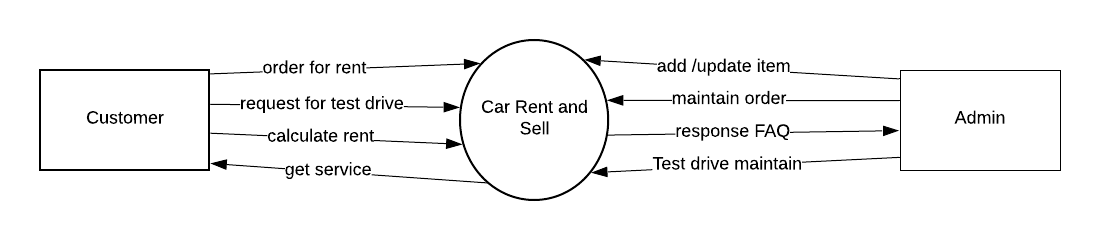
\includegraphics[width=6.00in, height=5.50in]{figures/C0}

\noindent 

\noindent 
{\bf Figure 3.1: Context Level diagram of Car Rent and Sell Website}
\end{figure}

\noindent 

\begin{figure}


\section{Level 1 Diagram}

\noindent A level 1 data flow diagram (DFD) is more detailed than a level 0 DFD but not as detailed as a level 2 DFD. It breaks down the main processes into subprocesses that can be analyzed and improved on a more intimate level.

\noindent The diagram of Level 1 is given below:\\


\noindent 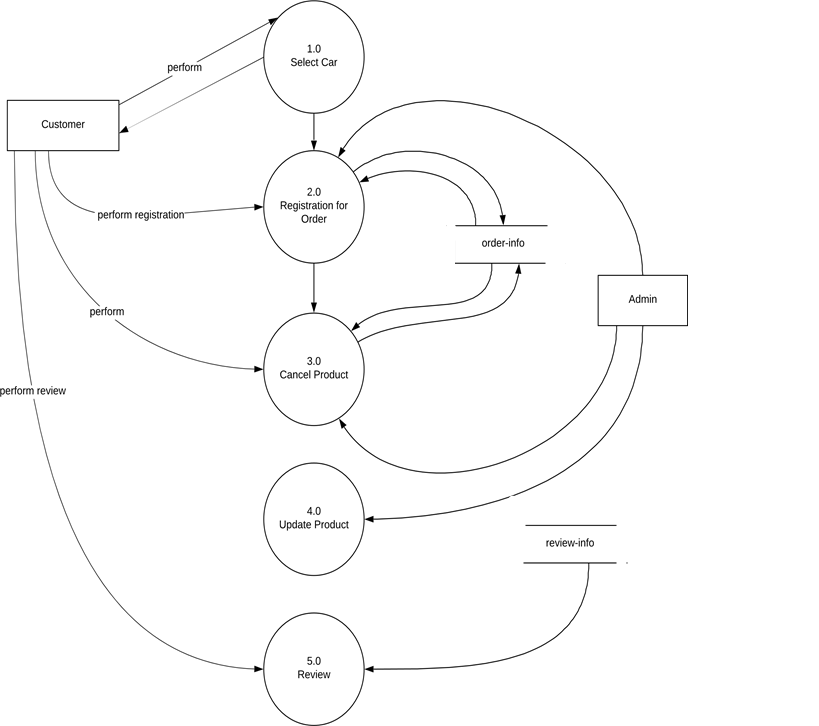
\includegraphics[width=5.50in, height=7.21in, keepaspectratio=false]{figures/C1}

\noindent 

\caption{Level 1 diagram of Car Rent and Sell Website}


\end{figure}


\noindent 
\begin{figure}


\section{Level 2 Diagram}

\noindent A level 2 data flow diagram (DFD) offers a more detailed look at the processes that make up an information system than a level 1 DFD does. It can be used to plan or record the specific makeup of a system.

\noindent \\


\textbf{1.Select Car Process:}


\noindent \textbf{}

\noindent 

\noindent The diagram of Select Car Process is given below:

\noindent 

\noindent \includegraphics*[width=5.70in, height=3.17in, keepaspectratio=false]{figures/SelectCar}

\noindent 

\caption{Select Car Process of Car Rent and Sell Website}
\end{figure}
\noindent 

\noindent 

\noindent 
\begin{figure}



 \textbf{2.Registration for Order Process:}


\noindent 

\noindent The diagram of Registration for Order Process of Car Rent and Sell Website is given below:

\noindent 

\noindent \includegraphics*[width=6.50in, height=3.50in, keepaspectratio=false]{figures/Registration}
\caption{Registration for Car Process of Car Rent and Sell Website}
\end{figure}
\noindent 

\noindent 

\noindent 

\noindent 

\noindent 

\noindent 
\begin{figure}


 \textbf{3.Cancel Order Process:}


\noindent 

\noindent 

\noindent The diagram of Cancel Order Process of Car Rent and Sell Website is given below:

\noindent 

\noindent \includegraphics*[width=6.50in, height=3.33in, keepaspectratio=false]{figures/Cancel}
\caption{ Cancel Order Process of Car Rent and Sell Website}
\end{figure}
\noindent 

\noindent 
\begin{figure}


 \textbf{4.Update Order Process}


\noindent 

\noindent 

\noindent 

\noindent The diagram of Update Order Process of Car Rent and Sell Website is given below:

\noindent 

\noindent \includegraphics*[width=5.50in, height=3in, keepaspectratio=false]{figures/Update}

\caption{Update Order Process of Car Rent and Sell Website}
\end{figure}
\noindent 

\noindent 
\begin{figure}

 \textbf{5.Review}


\noindent 

\noindent The diagram of Review Process of Car Rent and Sell Website is given below:

\noindent \includegraphics*[width=5.50in, height=3in, keepaspectratio=false]{figures/Review}

\caption{ Review Process of Car Rent and Sell Website}
\end{figure}
\noindent 

\noindent 

\noindent 


\begin{figure}

\section{Use Case Diagram}

\noindent A Use Case model defines what a system does without describing how the system does it. This logical model of the system replicates the understanding of a system from the viewpoint of a user outside the system, which is the system's requirement. It also splits the mode of the system that works into actions, services and reactions that are major to the users of the system.


\subsection{Actors}

\textbf{Customer: }Customers can select car, ask for test drive, rent car, cancel orders.\newline
\textbf{Admin: }Admin can manage registration process, update products and make orders decisions.

\subsection{Details of Use Case Models}

\noindent In Car Rent and Sell Website, we have the following use cases for these two actors:

\noindent \textbf{\underbar {Select Car}}

\noindent Actor: Customer
\noindent Primary Path:

\begin{enumerate}
\item  Check availability.

\item  Select required car. 
\end{enumerate}

\noindent \textbf{\underbar {Registration for Order}}

\noindent Actor: Customer
\noindent Primary Path:

\begin{enumerate}
\item  Collect customer’s info.

\item  Verify customer. 
\end{enumerate}

\noindent Alternative Path:
\begin{enumerate}
\item  In case of failure display registration error.

\end{enumerate}

\noindent \textbf{\underbar {Cancel Order}}

\noindent Actor: Customer
\noindent Primary Path:

\begin{enumerate}
\item  Confirm Cancellation

\end{enumerate}


\noindent \textbf{\underbar {Update Product}}

\noindent Actor: Admin
\noindent Primary Path:

\begin{enumerate}
\item  Add new car.

\item  Remove unavailable car.

\item  Update rent price and selling price.
\end{enumerate}


\noindent Alternative Path:
\begin{enumerate}
\item  Can’t update due to some unexpected reason.

\end{enumerate}


\noindent \textbf{\underbar {Review}}

\noindent Actor: Customer
\noindent Primary Path:

\begin{enumerate}
\item  Can review rent service.

\item  Can review sell service.

\end{enumerate}

\end{figure}

\begin{figure}

\subsection*{Use Case Relationships}

\noindent The final element in Use Case diagrams are Relationships. There are 4 types of relationships:

\noindent 
\subsection{Association}

\noindent An association between an actor and a use case specifies that the actor and the use case in some way interact or communicate with each other. In this relationship, an actor is connected to a use case using line with no arrowheads.


\noindent 
\subsection{Include}

\noindent Between 2 use cases include is a directed relationship, used to show that performance of the included use case is inserted into the behavior of the including (base) use case. Usually a use case comprises a behavior that is common to more than one other use case. Here, the arrow directs to the common use case.


\subsection{Extend}

\noindent Extend identifies how \& when the behavior cleared in usually optional extending use case can be introduced into the behavior established in the extended use case. From the base use case, different use cases handle exceptions. The arrow plugs from the extended to the base use case.\textbf{}
\end{figure}
\begin{figure}

\noindent 
\subsection{Generalization/ Inheritance}

\noindent Generalization states the relationship that can happen between two use cases and shows that one use case (child case) inherits the structure, behavior and relationships of the another actor (parent). Here, the arrow points to the general use case (parent case).


\noindent 
\subsection*{Extension Points}

\noindent Use cases can include conditional steps as well as extensions or alternative scenarios. Extension point is a property of a use case that categorizes a point where the actions of a use case can be amplified with elements of another (extending) use case.



\noindent 


\section{Use Case Models}


\noindent \includegraphics*[width=5.51in, height=4 in]{figures/use}

\caption{Use Case Diagram for Car Rent and Sell Website}


\section{Conclusion}

\noindent As our project is Car Rent and Sell, the main intention behind this project is to provide such type of facilities which can prevent the wastage of time while buying car in the showroom and book a car for rental purpose. With the help of data flow diagram, we have achieved the clear idea about process on the system and relations among them. In use case diagram we have found the relationship among actors and entire system which will help to develop our project very clearly and smoothly.

\end{figure}